\chapter{系统设计}
\label{chap:SystemDesign}

系统设计主要包含系统异步调度的设计和模块化的设计。

\section{异步调度}

由于内核和用户的调度信息是通过ring\_scheduler共享的,因此ring\_ scheduler将会被放在内存的一个固定的空间上,通过一个起始地址,使得内核空间和用户空间可以访问相应的程序。以下是关于ring\_ scheduler的一些设计。

\subsection{ring\_scheduler}


ring\_scheduler中的黑盒调度任务池资源,同时为内核和用户提供一系列的数据接口,实现任务资源在内核态和用户态两者之间的统一调度。

\subsubsection{元数据}

元数据是ring\_scheduler基本的调度单位

\begin{itemize}
\item hart\_id: 运行该任务的硬件线程编号,简单化为核的ID号
\item address\_space\_id: 地址空间编号
\item task\_repr: 任务指针,由所在的地址空间解释为任务
\item state: 任务状态
\end{itemize}


address\_space\_id指示任务地址,在分页机制下,通过KernelHartInfo,取得地址空间的映射关系,找到任务执行的物理地址。

task\_repr是任务指针,内核空间和用户空间的任务在ring\_scheduler由其指代,同时只有当task\_repr通过正确的地址转换才能得到正确的任务结构。

如果任务指针在其他地址空间尝试被解析,那么极会触发缺页异常,即使发生转换,其数据也是未定义的,不合法的。得益于指令集设计上的地址空间隔离的作用,使得任务指针在实现上存在一定的安全性。


state标记这个任务的状态,至少会有两种状态的存在:就绪与睡眠。就绪状态的任务表示该任务的某个阶段已经准备好可以进一步执行;睡眠状态的任务表示该任务需要等待一些数据或者其他任务的完成,处于等待状态。

就绪状态的任务可以被ring\_scheduler弹出交给内核或用户运行,睡眠状态的任务只有被唤醒器唤醒之后才能转成就绪状态,然后被进一步执行。

\subsubsection{ring\_scheduler的接口}

\begin{lstlisting}[caption=调度器的接口约束]
pub trait Scheduler<T: Clone + PartialEq> {
    type Priority;
    fn add_task(&mut self, task: T) -> Option<T>;
    fn peek_next_task(&self) -> Option<&T>;
    fn peek_next_task_mut(&mut self) -> Option<&mut T>;
    fn next_task(&mut self) -> Option<T>;
    fn current_task(&self) -> Option<T>;
    fn remove_task(&mut self, task: &T);
    fn set_priority(&mut self, task: T, priority: Self::Priority);
    fn queue_len(&self) -> Option<usize> {
        None
    }
}
\end{lstlisting}


\begin{itemize}
\item add\_task:尝试向调度器中添加一个任务
\item peek\_next\_task:获取下一个任务不可变的引用
\item peek\_next\_task\_mut:获取下一个任务可变的引用
\item next\_task: 得到下一个任务
\item current\_task:获取正在运行的当前任务,在发生中断时,通过这个保存任务的上下文
\item remove\_task:从调度器中移除一个任务
\item set\_priority: 设置任务的优先级,没有实现
\item queue\_len:返回队列的长度,如果不存在,则返回None
\end{itemize}


\subsubsection{先来先服务的队列处理方式}

这里采用最简单的任务调度算法,ring\_scheduler的底层实现了一个循环队列用以存储相应的任务结构,和相应的一些操作。底层队列的长度将是固定的,当队列中的任务处于唤醒时或队列已经放不下相应任务时,ring\_scheduler会将相应任务弹出,对于后者则阻止新任务的队列加入。

\subsection{异步}

调度器和执行器是分离的。调度器只根据元数据调度,得到下一个任务是什么。而这个任务该如何运行,调度器不知道,需要交给执行器来解释元数据的意义,拿到异步结构之后运行。

\subsubsection{任务的状态}

\begin{equation}
    \label{equation:c3taskstate}
    \begin{aligned}
\boldsymbol{\mathrm{TaskState}} = (\mathrm{Ready}, \mathrm{Sleeping}, \mathrm{Finished})^{\mathrm{T}}
    \end{aligned}
\end{equation}

其中,任务有TaskRepr的指针传递进来, 其中如果状态为Ready时, 表示任务可以执行,应当被ring\_scheduler弹出。Sleeping则表示任务处于休眠状态, 当ring\_scheduler中的任务睡眠的程度到达内核约束的值或,应当由内核通过一定方式尝试唤醒适量的任务。最后, Finished则表示任务已经完成。

\subsubsection{共享的数据}

参考元数据, $\boldsymbol{\mathrm{Task}} := (\mathrm{hartId}, \mathrm{addressSpaceId}, \mathrm{taskRepr}, \mathrm{State})^{\mathrm{T}}$。为了使得内核和用户态的任务可以得到共享,因此内核态和用户态的任务都应当有如下描述:

\begin{lstlisting}
struct Task {
    pub id: TaskId,
    pub process: Arc<Process>,
    pub inner: Mutex<TaskInner>,
    pub future: Mutex<Pin<Box<dyn Future<Output = ()> + 'static + Send + Sync>>>, 
}
\end{lstlisting}

\subsubsection{执行器的实现}

由于调度器和执行器是分离的,调度器只知道任务的运行状态,而不知道该如何对任务进行操作。因此后半部分的工作将需要执行器的介入,而执行器的工作依赖于调度器的返回,若执行器返回遵循以下的规则

\begin{equation}
    \label{equation:c3schedulerreturn}
    \begin{aligned}
\boldsymbol{\mathrm{SchedulerReturn}} = (\mathrm{TaskRepr}, \mathrm{SholdYield}, \mathrm{NoWakeTask}, \mathrm{Finished})^{\mathrm{T}}
    \end{aligned}
\end{equation}

其中

\begin{itemize}
    \item TaskRepr, 应当立即执行特定任务, 执行器从调度器获得这个值的时候需要调用相关方法释放任务,如果不释放任务,再次执行,还是会得到相同的任务。
    \item ShouldYield, 其他地址空间的任务要运行,应当提示执行器主动让出,并携带下一个地址空间信息。与此同时用户态应该执行yield,保存当前用户上下文,并切换至内核转到下一个地址空间。
    \item  NoWakeTask,调度器里面没有醒着的任务,但存在睡眠的任务。
    \item  Finished,队列已空,所有任务已经结束。
\end{itemize}


内核执行器的设计

在一个大循环中,不断从共享调度器中拿到任务,对任务进行poll操作,如果返回Ready,从共享调度器中删除该任务,如果返回Pending,将该任务设置为睡眠状态。如果共享调度器中所有任务都已完成,则退出系统。

\begin{lstlisting}[caption=内核执行器的设计]
pub fn run_until_idle() {
    loop {
        let task = peek_task(); // 从共享调度器中拿出下一个任务的指针,不弹出
        match task {
            TaskResult::Task(task_repr: usize) => { // 任务指针
                set_task_state(task_repr, TaskState::Sleeping); // 设置任务的状态为睡眠
                let task: Arc<KernelTask> = unsafe { Arc::from_raw(task_repr as *mut _) };
                // 注册 waker
                let waker = waker_ref(&task);
                let mut context = Context::from_waker(&*waker);
                let ret = task.future.lock().as_mut().poll(&mut context);
                if let Poll::Pending = ret {
                    core::mem::forget(task); // 不要释放task的内存,它将继续保存在内存中被使用
                } else {
                    // 否则,从共享调度器中删除此任务
                    delete_task(task_repr);
                } // 隐含一个drop(task)
            },
            TaskResult::ShouldYield(next_asid: usize) => {...}, // 不同地址空间的任务,需要切换地址空间
            TaskResult::NoWakeTask => {...},
            TaskResult::Finished => {...}
        }
    }
}
\end{lstlisting}

用户执行器的设计

用户执行器的设计和内核执行器存在一点区别,就是当拿到不在当前地址空间的任务的时候,不释放这个任务的内存,执行切换地址空间的系统调用。

\begin{lstlisting}[caption=用户执行器的设计]
pub fn run_until_idle() {
    loop {
        let task = peek_task(); // 从共享调度器中拿出下一个任务的指针,不弹出
        match task {
            TaskResult::Task(task_repr: usize) => {...},
            TaskResult::ShouldYield(next_asid: usize) => {
                mem::forget(task);
                do_yield(next_asid);
            },
            TaskResult::NoWakeTask => {...},
            TaskResult::Finished => {...}
        }
    }
}
\end{lstlisting}

\section{模块设计}

为了简化系统开发的压力和提高系统升级的灵活性,模块化无疑是比较好的选择,本文提出静态模块化设计和动态模块化设。前者依赖与开发语言的编译时模型,将一些API层面上的接口给正交开的,形成各自独立的模块,彼此之间互相独立,各自又通过API的接口调用形成自己的调用规范,从而可以独立于系统内核供给其他项目使用。而后者则是在静态模块化工作基础上的一个延申,动态的模块化依赖语言的运行时模型,每一个运行时的独立单元都会被抽象为一个可悲装载和卸载的模块单元,这样就会大大提高内核升级的灵活性。

\subsection{静态模块}

在静态模块的设计中,系统模块设计应当遵循以下原则:

\begin{enumerate}
    \item 最小正交化的模块
    \item 树状依赖和空间隔离
\end{enumerate}

\subsubsection{最小正交的模块}


\begin{figure}[htb]
    \figureCapSet
    \centering
    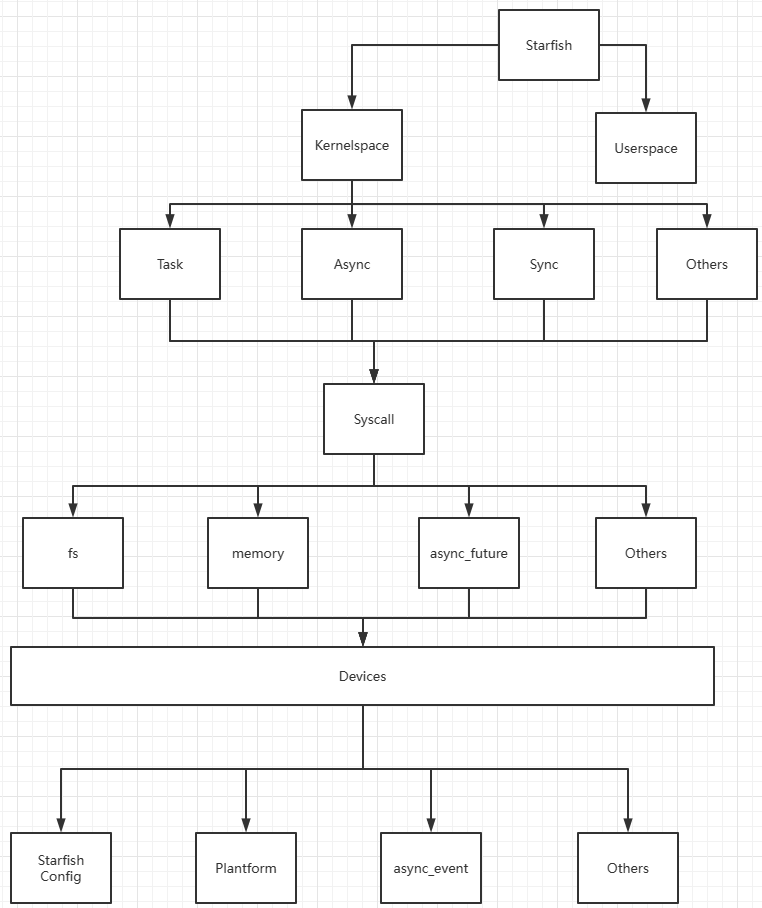
\includegraphics[width=.8\linewidth]{figure/c3/starfishstructure.png}
    \caption{Starfish 的静态模块分解图}
    \label{figure:c3starfishstructure}
\end{figure}

参考\autoref{figure:c3starfishstructure},这是最开始设计的内核模块的静态的拆分图。为了方便描述,每一层定义为抽象层级,处在最底层的其抽象层级为0,层级越低抽象的能力越小,反之则越大。而每一层的节点可以定义为抽象因子。例如,Starfish Config为0层的抽象因子,其寓意为在该层级的最小正交因子(即在当前的抽象下,该因子为最小的不可再分割的正交参考)。

正交,顾名思义就是将一个复杂的“合力”,通过相应的参考系,进行有序分解,形成一个可以通过参考系中的相应因子描述的矢量,例如 $\boldsymbol {v}=(a, b)$, 则可以准确表述矢量$\boldsymbol {v}$在直角坐标系中的空间表示。

类比前者,提出抽象正交化的概念,我们将整个抽象空间则概括为由抽象层级和抽象因子组成的抽象评估空间,其空间的单位为抽象评估因子,则可以得到如下式子,


\begin{equation}
    \label{equation:c3elf}
    \begin{aligned}
       \boldsymbol{\mathrm{E}} = (L, F)
    \end{aligned}
\end{equation}

其中$\boldsymbol{E}$表示评估因子,L表示抽象层级,F表示抽象因子。由此可以总结出两组概念:最小正交化和严格最小正交化。

\begin{enumerate}
    \item 最小正交化: 当$L=0$时,即抽象层级为0,即模块不可再分的情况下, $\boldsymbol{E}$为最小正交化的评估因子,此时模块分解为最小正交化。
    \item 严格最小正交化: 在满足最小正交化的前提下, 有$F = {F_{0}, F_{1}, \cdots, F_{n}}$,其中$0 = {F_{0} \cap F_{1} \cap \cdots \cap F_{n}}$, 此时, $\boldsymbol{E}$为严格正交化的评估因子,此时模块分解为严格最小正交化。
\end{enumerate}

当$\boldsymbol{E}$为严格正交化时,则可以说模块分解达到了一个最优的状态,此时所有的$L=0$级的模块之间不存在互相干扰的情况,彼此之间的联系,仅仅通过语言编程者之间的API约束,如此的好处可以使得模块之间的耦合程度变低,相互之间可以独立进行开发,同时如果他人的内核也遵循了相应的API约束,则该模块可以达到共享的目的。


\subsubsection{树状依赖和空间隔离}


通过\autoref{figure:c3starfishstructure}的观察,可以发现模块的分解和组合,其静态的模块将会形成一种树状的结果,此时L(即抽象层级)之间是存在“方向”的,即当存在$L_{i} < L_{j} (i < j)$时, $L_{j}$必然是由部分$L_{i}$组成,而必不可能存在上下互换的生成形式,如若L的层级方向出现错误,则$\boldsymbol{E}$将无法做出评估,其模块拆解也必然是错误的。由此,一个良好的模块分解必然会形成一个层次分明的树状依赖。

当L一定, $F = {F_{0}, F_{1}, \cdots, F_{n}}$时, 若有$0 = {F_{0} \cap F_{1} \cap \cdots \cap F_{n}}$,此时的$\boldsymbol{E}$可以达到最优解,即优化评估因子,记作$\boldsymbol{OE}$,特别地当 $L = 0$时,若形成$\boldsymbol{OE}$,即$F$达到分解地最优解,则此时就可以称为严格最小正交化。

其中$\boldsymbol{OE}$的意义是,层级间的依赖被解除,模块是独立,没有相互干扰, 可以达到层级空间间的空间隔离。同样以此可以逆向评估底层模块的$\boldsymbol{E}$特性, 通过数学归纳法,我们可以显而易见的得出当$L_{i} < L_{j} (i < j)$, 若$L_{j}$达到了$\boldsymbol{OE}$,则$L_{i}$也应当是$\boldsymbol{OE}$的。

\subsection{动态模块}

在动态模块的设计中,系统的模块设计应当遵循以下三个原则: \begin{enumerate}
    \item 需要获取所有模块的运行时的持久边界
    \item 最大限度地发挥语言(Rust)和编译器的作用
    \item 最小化模块之间的状态溢出
\end{enumerate}

\subsubsection{需要获取所有模块的运行时的持久边界}

系统内核中的模块组件具有明确定义的边界(严格化的正交模块),并在整个运行时保持不变: 在实现时,系统模块组件以Rust独立的Crate的形式存在;在编译时,系统模块组件以一组加载的内存区域的形式存在;在运行时,系统模块组件以一组加载内存区域的形式存在,内存区域具有每部分的边界和依赖元数据。

上述的设计原则每一个内核的系统模块组件都需要遵循。运行时,可以显示识别系统模块组件的边界是系统内核中组件隔离和状态管理的基础。

在运行时,系统内核根据需要将所有系统模块组件加载并链接到系统中。简而言之,这需要找到并解析系统模块组件对象,将其部分加载到内存中,解析其依赖,根据依赖树,以写入连接器重定位条目,根据需要递归加载任何丢失的系统模块组件,并向符号映射添加新的公共符号。基于此可以为内核进化和故障恢复提供理论基础。加载的系统模块组件集定义了一个系统模块组件空间,一个包含所有系统模块组件公共符号的真正的名称空间,用于快速解析单元格之间的依赖关系。每个加载的系统模块组件节点跟踪其组成部分和存储区域包含它们。每个系统模块组件中的部分对应于其Crate的目标文件中的部分,例如,可执行文件、只读数据和读写数据部分。每个加载的分段节点跟踪其大小、在存储器中的位置以及双向依赖性(输入和输出);额外的元数据用于加速系统模块组件交换和其他系统功能。

系统模块组件边界的持久性降低了复杂性: 系统内核的持久性系统模块组件边界在其存在的所有阶段提供了一致的系统结构抽象。这将会降低了开发者对系统的理想模型的复杂性,并简化了故障恢复和演化逻辑,因为系统内核可以在运行时从相同的面向系统模块组件的角度自省和管理它自己的代码。从顶层应用程序和库到核心内核组件的一切都可以作为系统模块组件来观察。这使得系统内核能够

\begin{itemize}
	\item 实现统一适用于任何单元的单一机制,即模块交换,以及
	\item 以安全的方式从多个系统层(例如,应用和内核组件)联合进化模块。
\end{itemize}

\subsubsection{最大限度地发挥语言(Rust)和编译器的作用}
通过使编译器能够最大限度地检查安全性和正确性不变量来最大限度发挥语言的力量。

将系统内核的执行环境与该语言的运行时模型相匹配,并在Rust等现代语言提供的强大的静态类型系统中实现操作系统概念。这将编译器检查的不变量(例如,没有悬空引用)扩展到了所有类型的资源,而不仅仅是语言中内置的那些。

依赖语言设计有两个主要好处:

\begin{itemize}
    \item 首先,它使编译器能够接管资源管理职责,减少了操作系统必须维护的状态,从而减少了状态溢出并加强了隔离。
    \item 它使编译器能够在理解代码行为的过程中应用安全检查,从应用程序到核心内核组件实现端到端安全,并将语义运行时错误转化为编译时错误。
\end{itemize}

相比之下,传统的非语言方法依赖于硬件保护和运行时检查来维护安全性、隔离性和正确性的不变量。这些特性对编译器是透明的,需要不安全的代码。甚至现有的安全语言操作系统。在语言级别的安全代码和底层的不安全核心之间有一个缺口,后者将语言所需的抽象实现为一个黑盒。

\subsubsection{最小化模块之间的状态溢出}

由于系统内核的组件结构是模块化的,因此状态溢出只能发生在跨越模块边界并导致接收单元状态改变的交互(例如,函数调用)中。
